% Author: Pranshu Bansal
% Email: pranshu@berkeley.edu
\note{
Description: derive intuition behind Ohm's law and I-V plots for resistors.
}

\begin{enumerate}

\item{In the graph below, plot the equation $y = 2x + 1$.
\begin{center}
    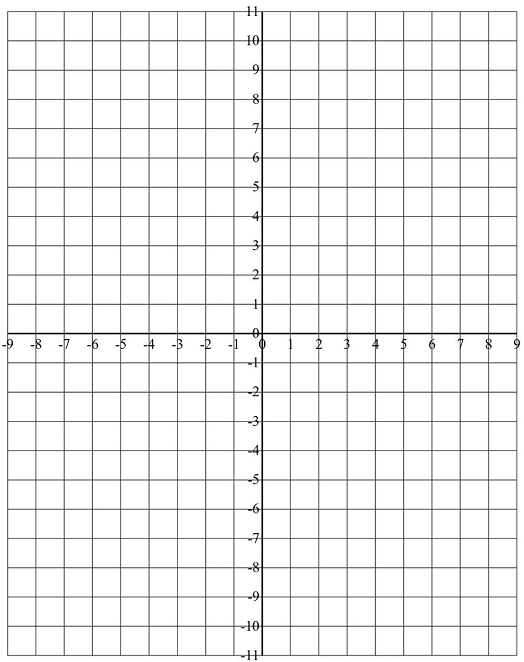
\includegraphics[scale=0.6]{../graph.png}
\end{center}
}

\sol{
\begin{center}
    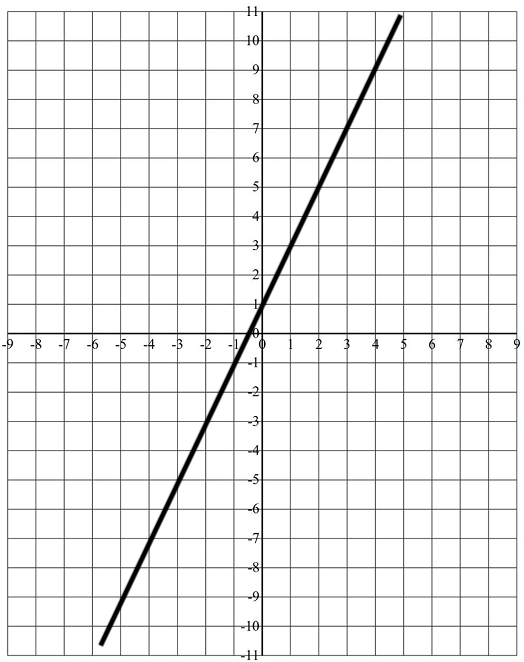
\includegraphics[scale=0.6]{../graph_sol1.png}
\end{center}
}

\item{Can this graph represent the I-V relationship of some resistor? Why or why not?}
\sol{
    No, this graph cannot represent the I-V relationship of a resistor because it doesn't pass through the origin. The current through a resistor cannot be non-zero when the voltage across it is zero and vice versa.
}

\item{Plot $y = -x$? Can it represent the I-V relationship of some resistor? Why or why not?
\begin{center}
    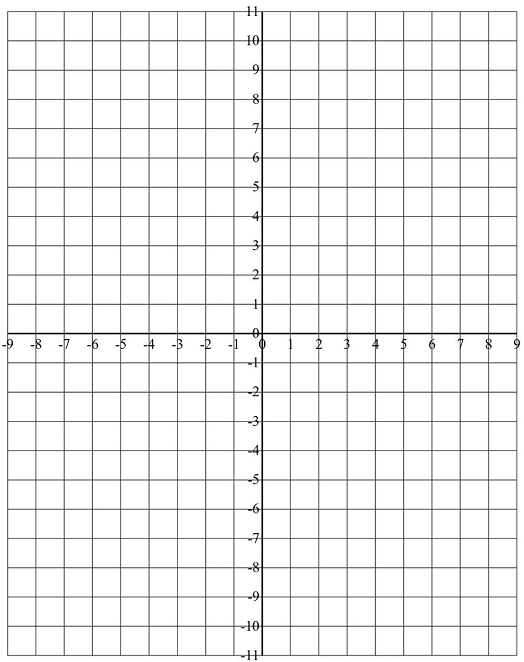
\includegraphics[scale=0.6]{../graph.png}
\end{center}
}
\sol{
\begin{center}
    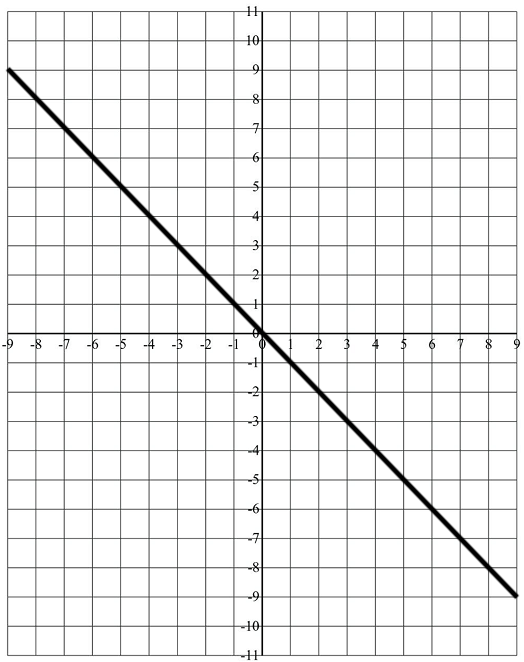
\includegraphics[scale=0.6]{../graph_sol2.png}
\end{center}
    
No. Even though this graph passes through the origin, it cannot represent the I-V relationship of a resistor because it passes through the second and fourth quadrant of the graph. The current through a resistor cannot be negative when the voltage across it is positive and vice versa.
}

\item{For a general linear equation, $y = mx + c$, what can you say about m and c for this equation to be the I-V relationship of a valid resistor?}

\sol{
For $y = mx + c$ to be a valid I-V relationship, two conditions must be satisfied. \\
The value of c has to be zero. This ensures that the current through a resistor cannot be non-zero when the voltage across it is zero and vice versa. \\
The value of m has to be positive. This ensures that the plot only passes through the first and the third quadrants. Hence, the voltage and the current always have the same sign.
}

\item{Can a non-linear polynomial be used to represent a resistor's I-V relationship?}

\sol{
    Ohm's law states that the relationship between the current through a resistor and the voltage across it is linear. Therefore, a non-linear polynomial cannot be used for such purpose.
}
\end{enumerate}
